\chapter{State of the Art \& Related Work}
\label{cha:chapter2}

This chapter provides an overview of the prominent solutions in the realm of blockchain scalability and introduces the foundational project upon which this thesis is built.

\section{Scalability Approaches}
Various strategies are being explored to enhance blockchain scalability. Some are already operational, while others are in the research stage. These strategies broadly fall into two categories: Layer 1 and Layer 2 solutions \cite{tyagi_study_2021,thibault_blockchain_2022}. Layer 1 solutions focus on boosting blockchain scalability through means like enlarging block sizes or implementing Sharding. In contrast, Layer 2 solutions endeavor to scale the blockchain by relocating computation off-chain. Noteworthy examples of Layer 2 solutions encompass State Channels, Sidechains, and Rollups, as illustrated in Figure \ref{fig:2_scalingSolutions}.

The prevailing trajectory for blockchain scalability involves the adoption of Layer 2 solutions. This course of action is being embraced by a significant portion of the Ethereum community \cite{neiheiser_practical_2023}.

\begin{figure}[ht]
  \centering
  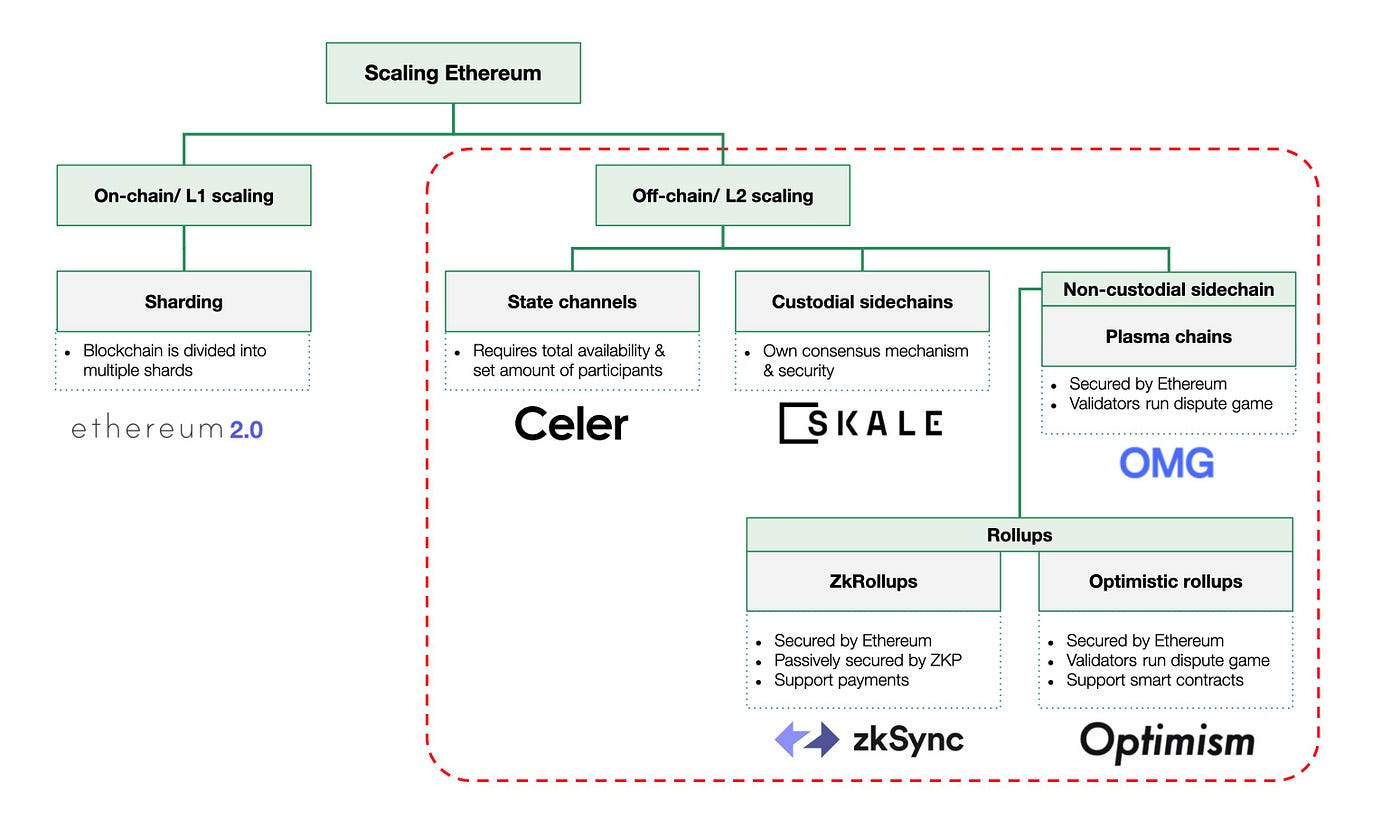
\includegraphics[width=0.95\columnwidth]{2_scalingSolutions.jpg}
  \caption[Scaling Solutions]{Principal scaling solutions for Layer 1 and Layer 2\footnotemark}  
  \label{fig:2_scalingSolutions}
\end{figure} 
\footnotetext{\url{https://medium.com/token-terminal/a-primer-on-ethereum-l2-scaling-techniques-17ac437891b1}}

\subsection{Zk-Rollups}
\label{sec:2_zkRollups}
Zk-Rollups represent a Layer 2 approach that leverages zero-knowledge proofs to conduct computation off-chain. Post-computation outcomes and a proof of verifiably correct execution are transmitted to the blockchain's smart contract. The smart contract then verifies the proof before incorporating the results onto the blockchain \cite{tyagi_study_2021}.

Figure \ref{fig:2_zkRollup_schema} outlines the Zk-Rollup paradigm. An user initiates a transaction with the off-chain node. The node processes the transaction batch, using the state fetched from the blockchain, and relays results and proof to the smart contract. Following proof validation, the new account balance list is recorded on the blockchain.

\begin{figure}[ht]
  \centering
  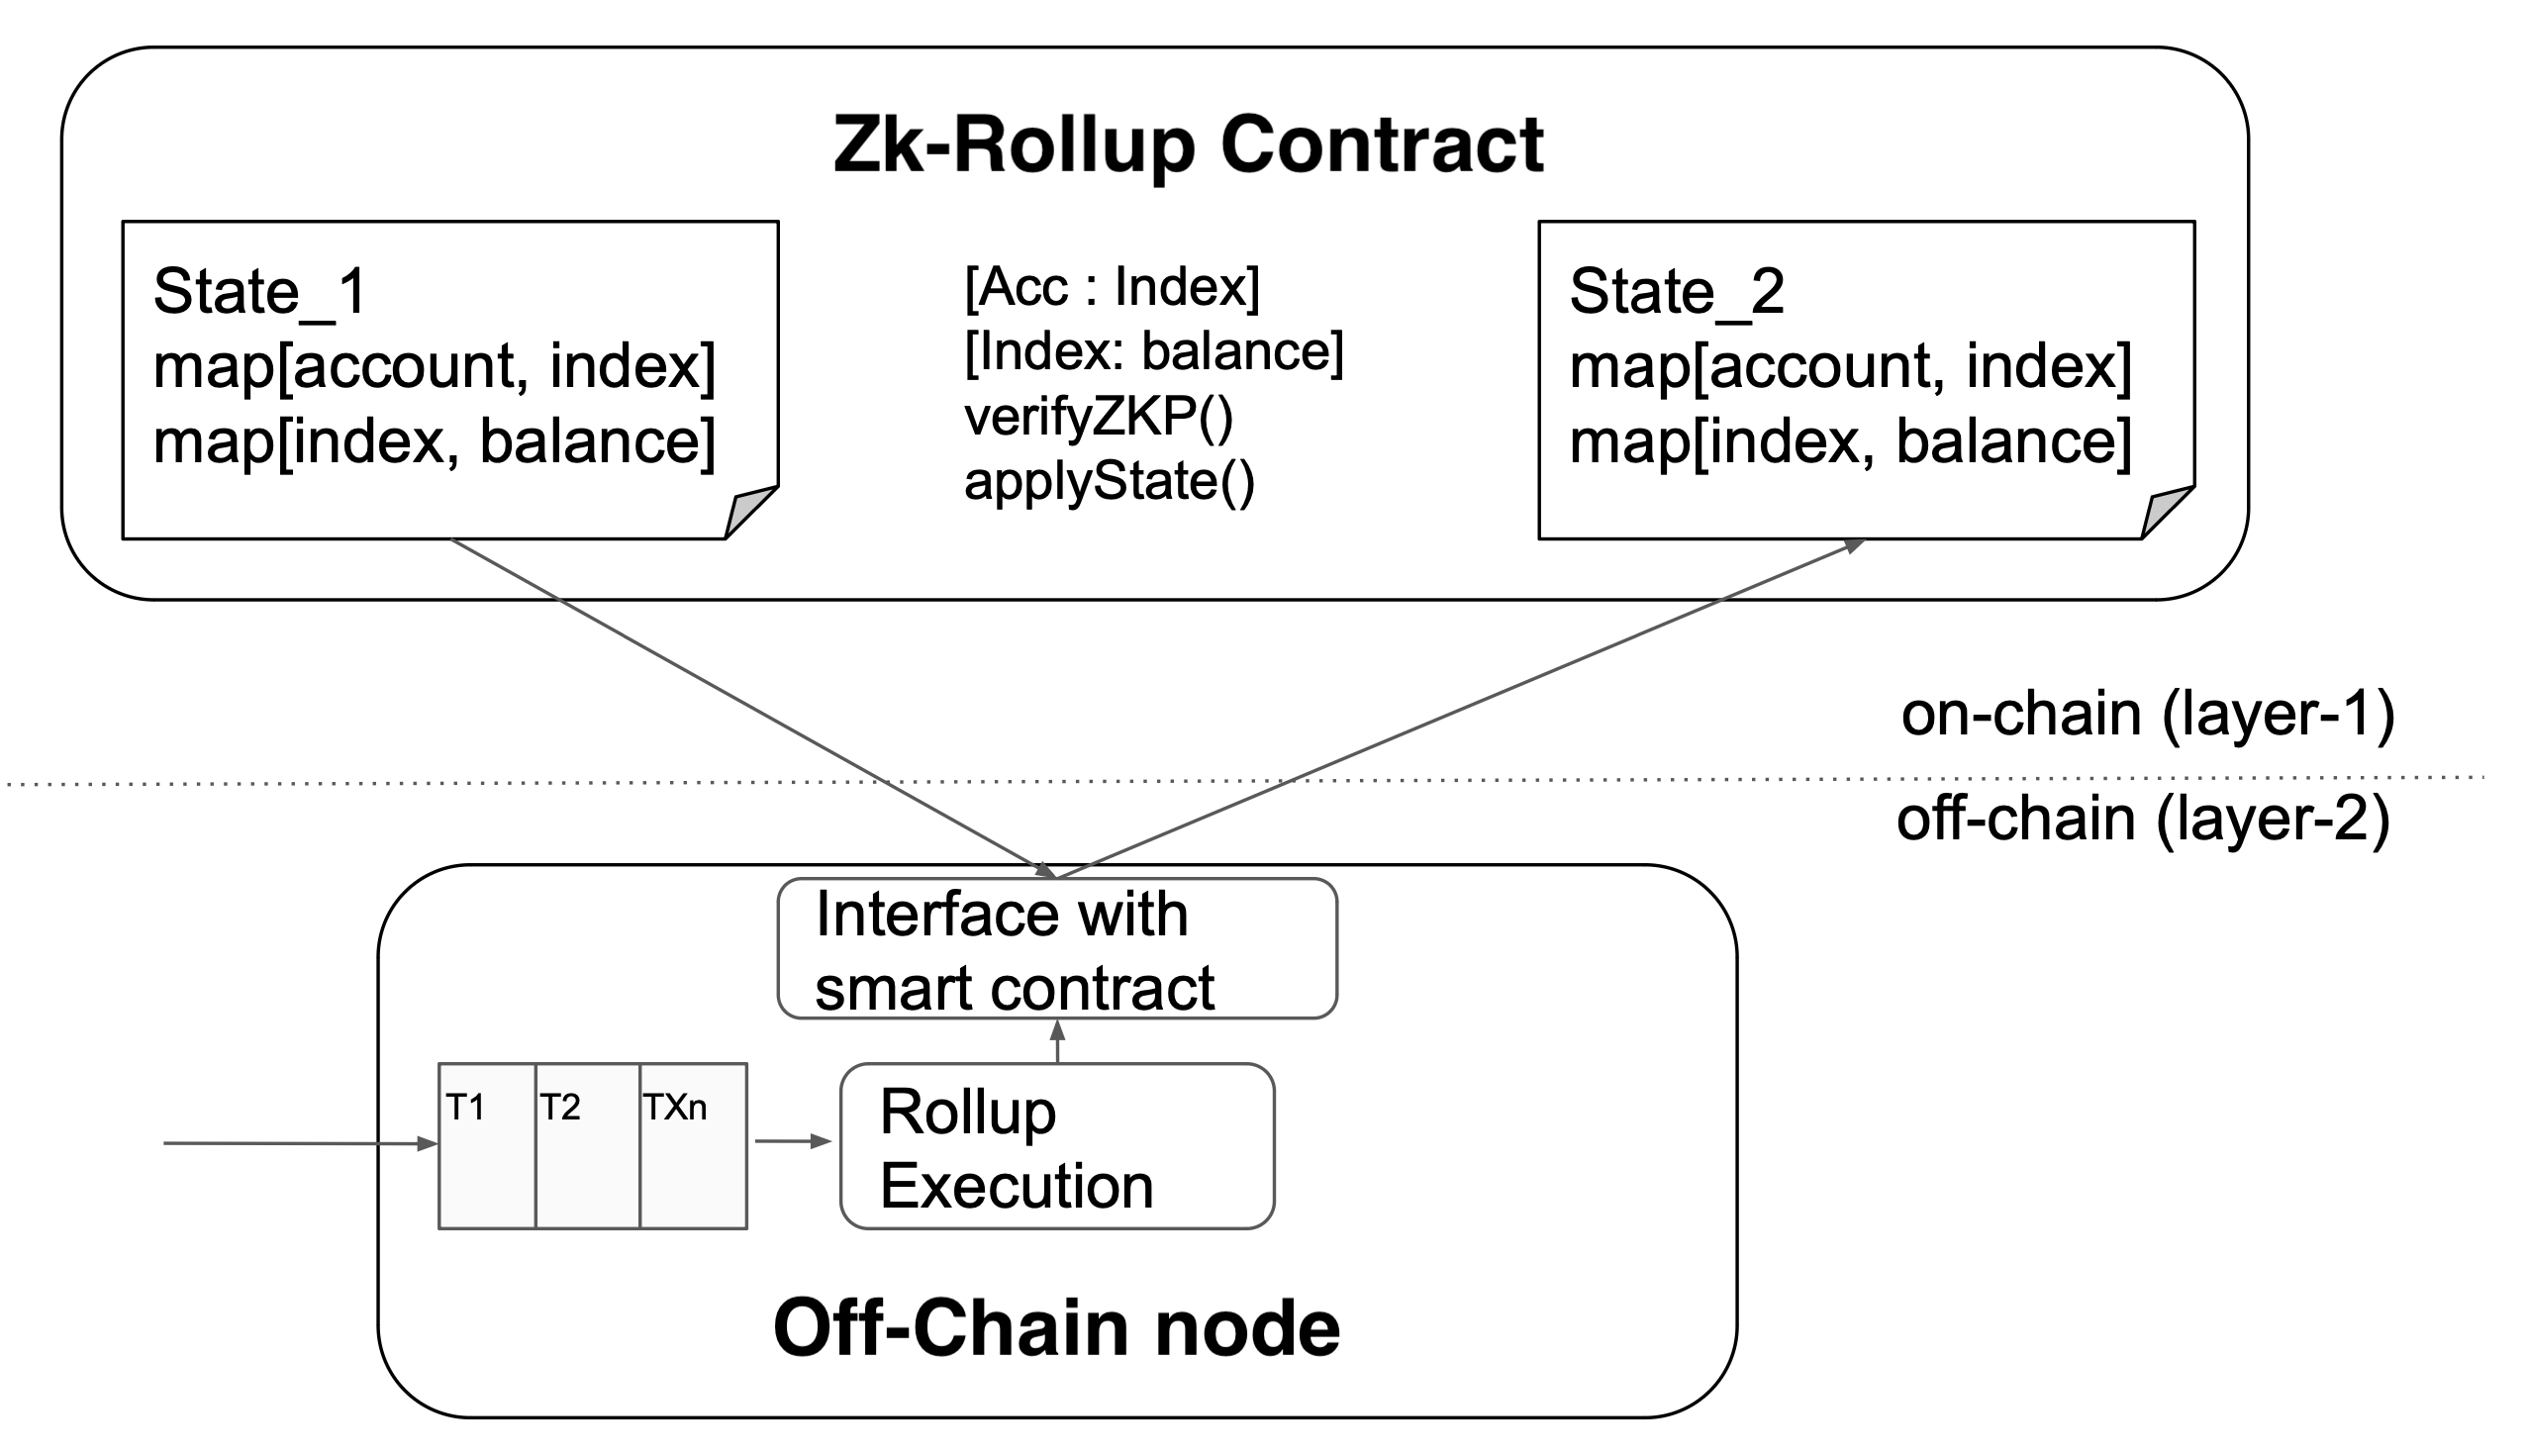
\includegraphics[width=0.95\columnwidth]{2_zkRollup_architecture.png}
  \caption[Zk-Rollup Schema]{General schema of a Zk-Rollup\cite{ise_department_tub_material_nodate}}  
  \label{fig:2_zkRollup_schema}
\end{figure}

\subsection{ZoKraStes}
ZoKrates is a toolbox for zkSNARKs on Ethereum: it allows developers to write zero-knowledge proofs in a high-level programming language and generate trusted setup parameters and zero-knowledge proofs \cite{eberhardt_ZoKrates_2018}.

\todo[inline]{explain ZoKrates}

\section{ADSP Project: Scaling Tezos Blockchain with Zk-Rollups \label{sec:2_adspProject}}
In the Winter Semester 2022/2023 at the University of Berlin, I collaborated with the ADSP (Advanced Distributed Systems Prototype) group on a project. The project's objective was to scale the Tezos blockchain using Zk-Rollups through the ZoKrates toolbox.

The group partially achieved the project's objectives, creating a proof of concept. The system architecture features Layer 1 and Layer 2 components: Layer 1 includes two smart contracts for state management and proof verification; Layer 2 encompasses a node executing transactions within the ZoKrates program, generating proofs for the smart contract. Figure \ref{fig:2_general_rollup_architecture} offers an overview of the entire system.

\begin{figure}[ht]
  \centering
  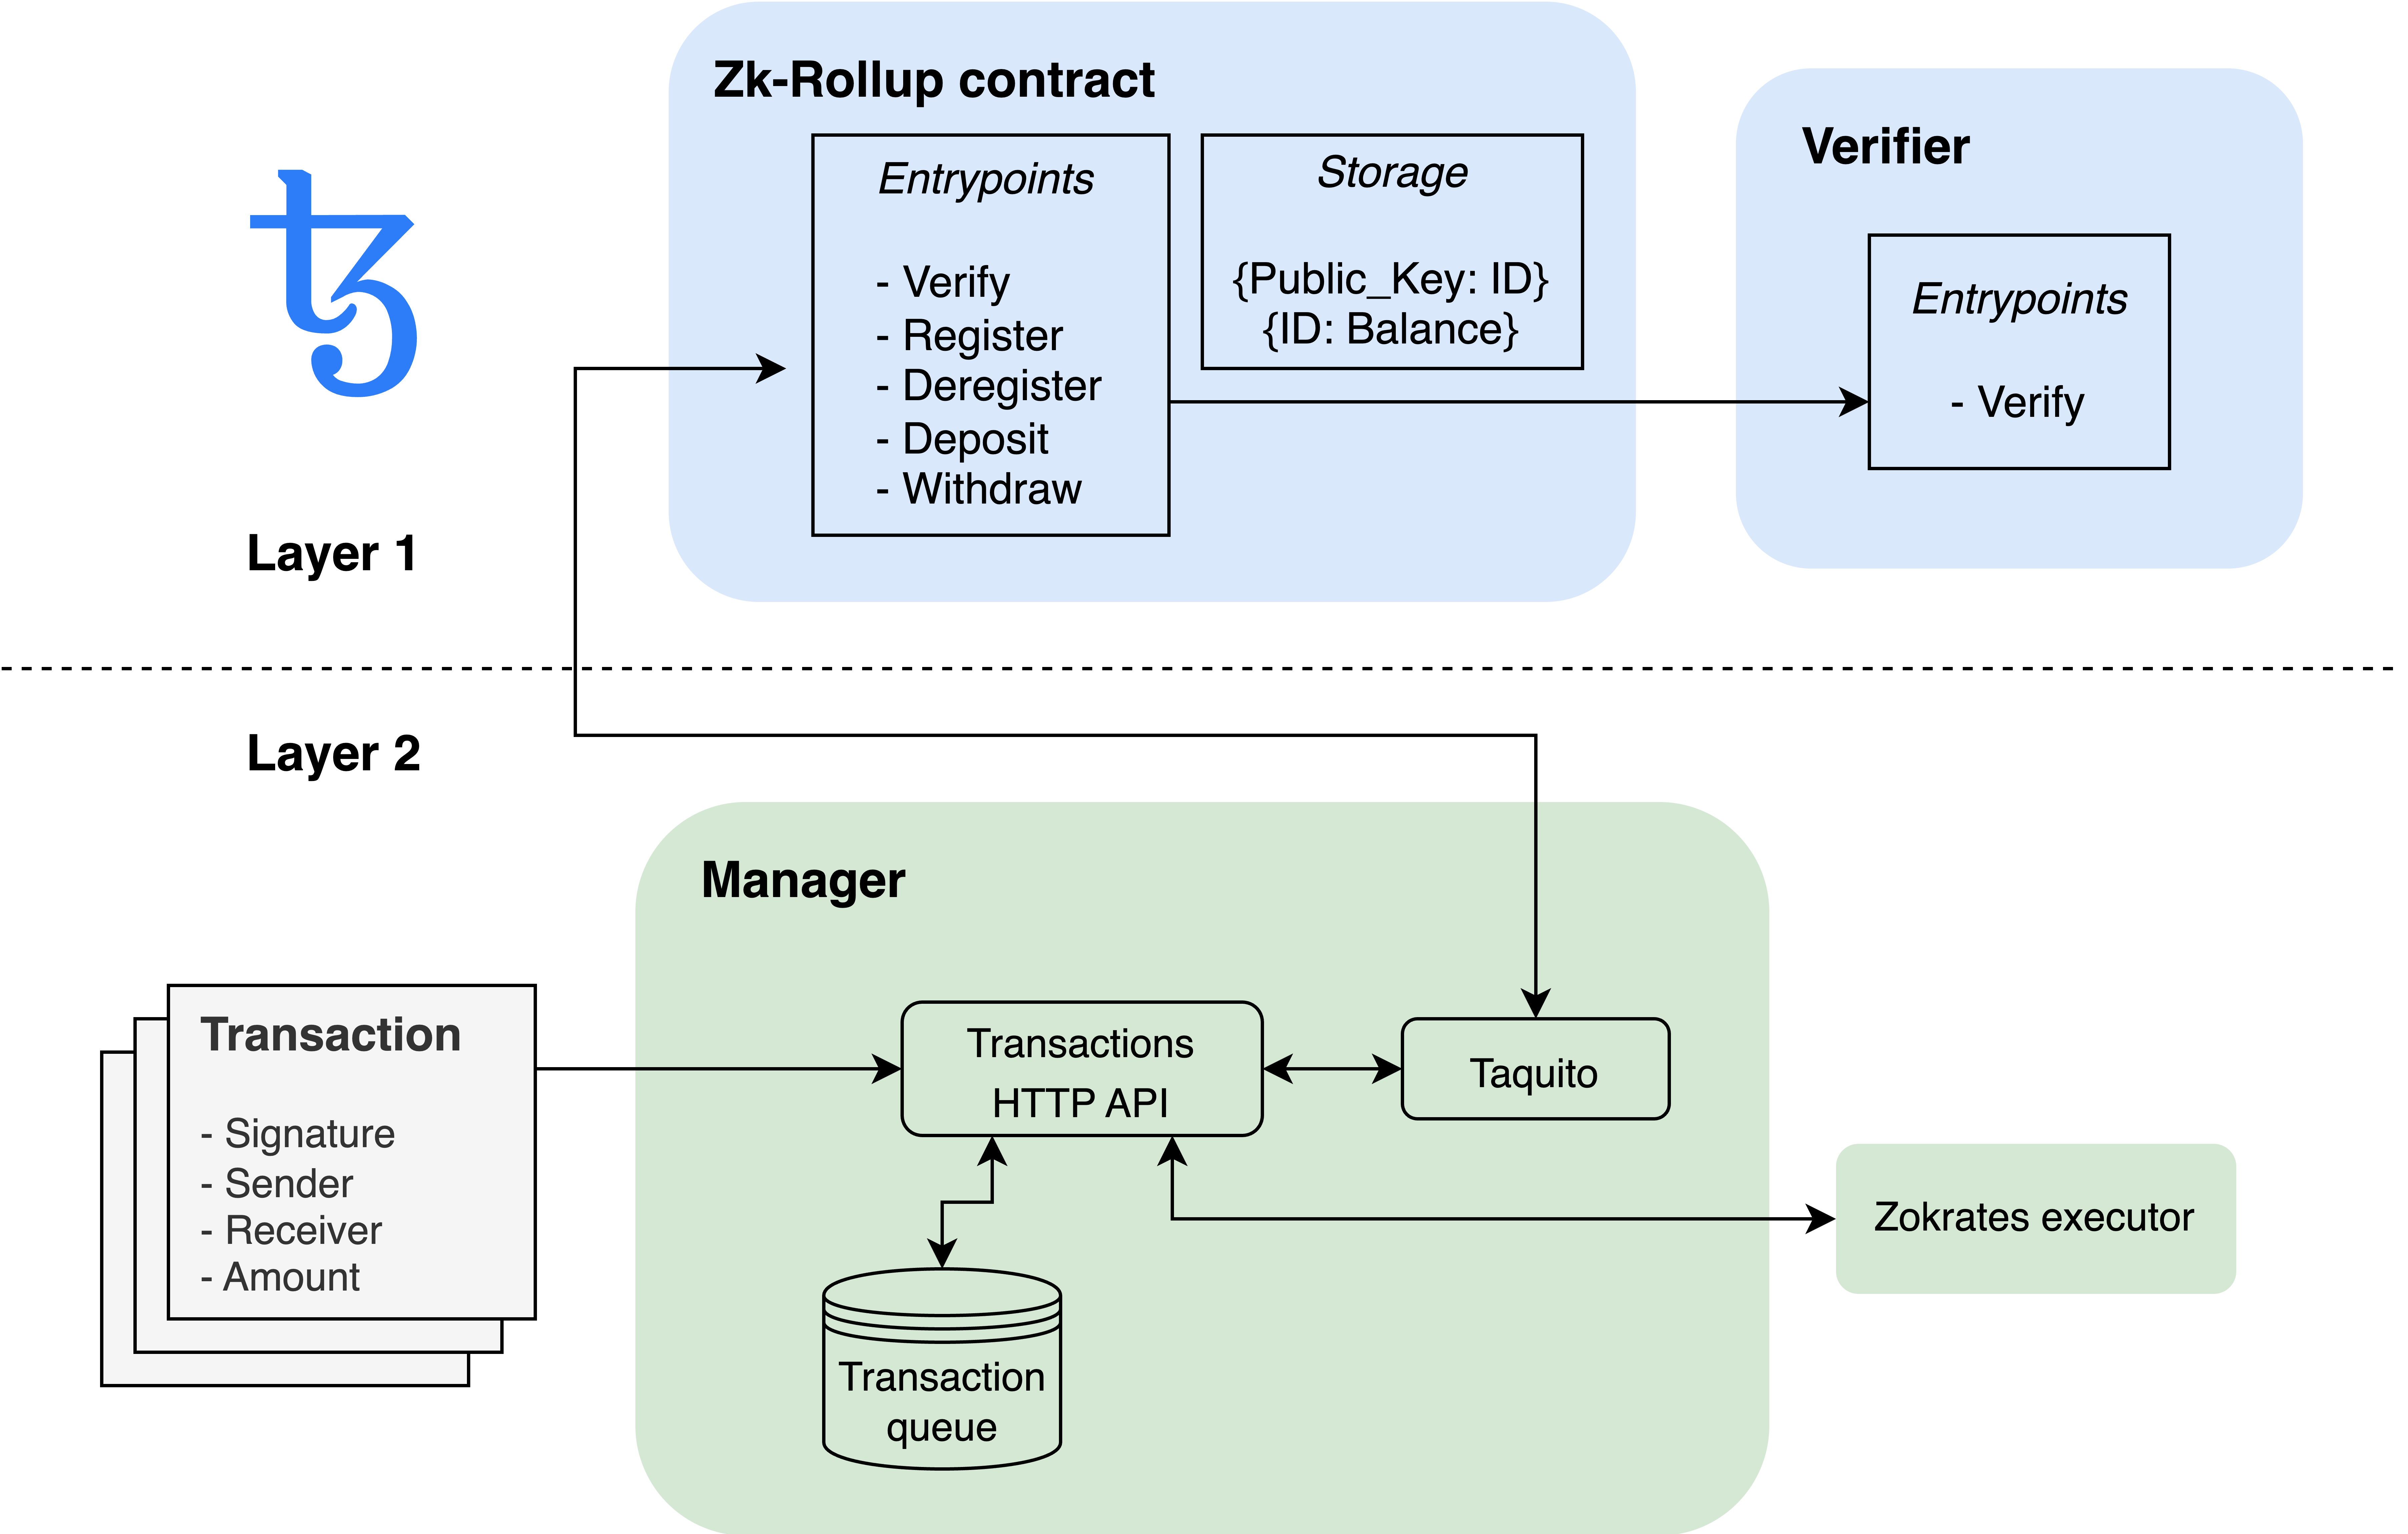
\includegraphics[width=0.95\columnwidth]{2_drawings-adsp_rollup_architecture.png}
  \caption[Zk-Rollup Architecture]{General Zk-Rollup architecture}  
  \label{fig:2_general_rollup_architecture}
\end{figure}

The Zk-Rollup execution process unfolds as follows:
\begin{enumerate}
    \item A user dispatches a transaction to the off-chain node, managed by a NodeJS server (the manager);
    \item The manager logs the transaction in a transaction queue;
    \item Once three transactions accumulate, the node processes the transaction batch, spawning the ZoKrates executor;
    \item The manager fetches the current state from the Tezos Zk-Rollup smart contract;
    \item The ZoKrates executor processes the ZoKrates program with the transaction batch and the current state as input;
    \item The ZoKrates executor generates a proof and new balance list, transmitting them to the NodeJS server;
    \item The NodeJS server converts ZoKrates outputs into a Tezos-compatible format;
    \item Converted outputs are dispatched to the Tezos Zk-Rollup smart contract using Taquito, an external library;
    \item The smart contract forwards the proof to the verifier smart contract;
    \item The verifier smart contract verifies the proof, communicating the result to the contract;
    \item If the proof is verified, the new balance list is stored in the Zk-Rollup contract's blockchain storage.
\end{enumerate}

Figure \ref{fig:2_drawings-adsp_sequence_general.png} illustrates the sequence of events in the Zk-Rollup execution process.

\begin{figure}[ht]
  \centering
  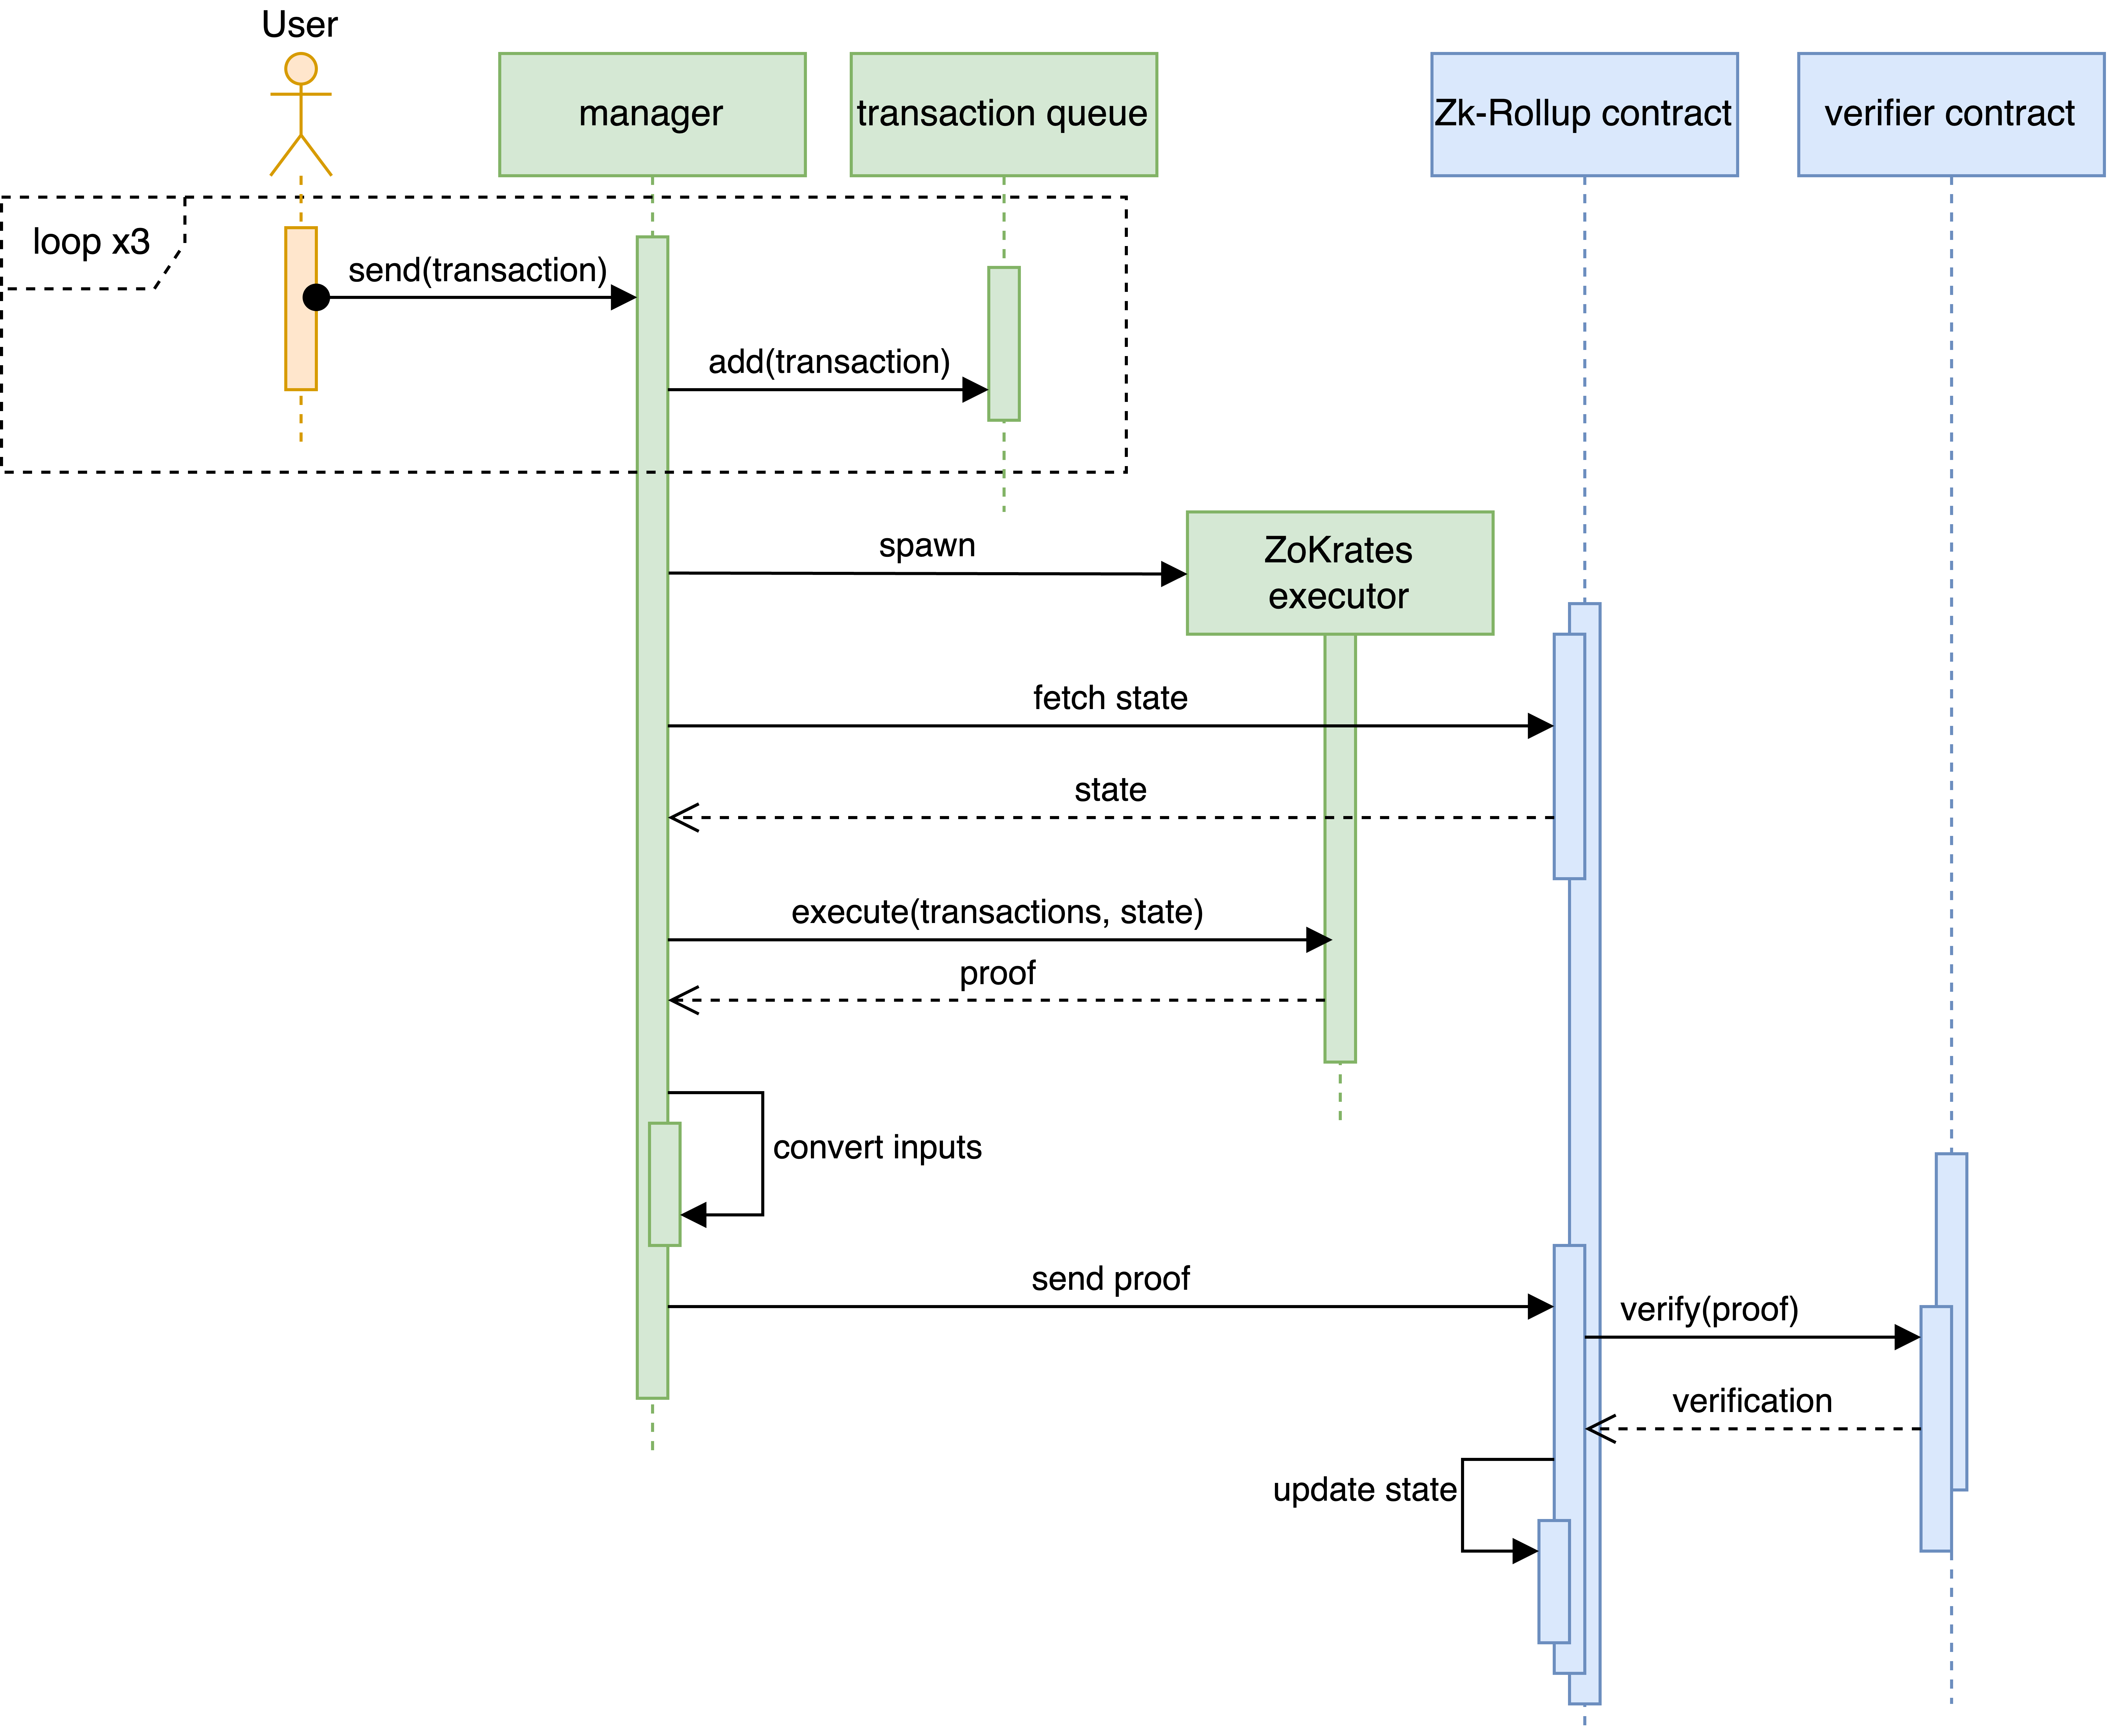
\includegraphics[width=1\columnwidth]{2_drawings-adsp_sequence_general.png}
  \caption[Sequence Zk-Rollup]{Sequence diagram of the Zk-Rollup execution process.}  
  \label{fig:2_drawings-adsp_sequence_general.png}
\end{figure} 

\subsection{Developed Components}
The team successfully implemented the Zk-Rollup \textit{Verify} entrypoint within the \textit{Zk-Rollup contract}, along with the \textit{NodeJS Manager}. Additionally, the storage mechanism was correctly executed.

The ZoKrates program was partially developed, including:
\begin{itemize}
    \item Verification of account inclusion in the rollup system;
    \item Verification of sufficient balance in sender account;
    \item Transaction execution;
    \item Generation of new balance merkle tree root, balance list, and proof.
\end{itemize}

The generation of the Merkle tree root is accomplished through the algorithm described below. This process utilizes the SHA2-256 hash function with automatic zero-padding. The algorithm incorporates pre-calculated values for the Merkle tree depth and the number of leaf nodes.

\noindent\textbf{Algorithm 1: Merkle Tree Root Generation}
\begin{lstlisting}[language=Python]
for i in 0...TREE_DEPTH {
  step_size = 2 ** (i + 1)
  step_number = LEAFS_NUM / step_size
  for j in 0...step_number {
    leftIndex = j * step_size
    rightIndex = leftIndex + step_size / 2
    leafs[leftIndex] = hash(
        leafs[leftIndex],
        leafs[rightIndex]
    )
  }
}
return leafs[0]
\end{lstlisting}

\subsection{Pending Components\label{subsec:pendingcomponents}}
Numerous aspects of the project remain unfinished, including:
\begin{itemize}
  \item Registration entrypoint;
  \item Deregistration entrypoint;
  \item Deposit entrypoint;
  \item Withdrawal entrypoint;
  \item Integration of signature checks within the ZoKrates program;
  \item Addressing the double spending issue;
  \item System optimization.
\end{itemize}
Furthermore, the project lacks a benchmarking study, a security analysis, and a cost comparison with alternative scaling solutions and Layer 1.

\todo[inline]{Provide a more comprehensive analysis of the project's state of the art.}

\section{Other Zk-Rollup Implementations}
Numerous Zk-Rollup implementations exist, particularly for Ethereum. The implementation discussed in \cite{dinh_implementation_2023} shares similarities with the ADSP project's approach. However, it lacks considerations for system scaling and handling multiple token types. Another example is Polygon Zero\footnote{\url{https://polygon.technology/blog/introducing-plonky2}}, which facilitates parallel execution of transactions on L2. This system blends STARK and SNARK, differing from the approach outlined in this thesis.

\section{Zk-Rollup Reviews}
Several studies have assessed the viability and performance of the Zk-Rollup system. \cite{capko_state_2022} offers an overview of prevalent zero-knowledge proofs. The ZoKrates Toolbox, utilized by the ADSP project, employs SNARK, which requires a trusted setup phase—a potential drawback compared to Transparent zk-SNARK \cite{zhou_overview_2022}. \cite{neiheiser_practical_2023} highlights the scalability bottleneck L2 solutions face due to slow L1, constraining them below theoretical L2 throughput. \cite{starkware_fractal_2021} proposes L3 to circumvent this issue.

\section{Alternative L2 Solutions}
Several Layer 2 strategies exist to scale blockchains. A brief overview follows.

Plasma: Plasma facilitates off-chain transaction processing through child chains or sidechains, connected to the main blockchain for security. Plasma chains expedite transactions but necessitate dispute resolution for potentially fraudulent actions \cite{thibault_blockchain_2022}. OMG Network\footnote{\url{https://docs.omg.network}} exemplifies a network employing Plasma.

State Channels: Off-chain payment channels, like state channels, enable direct user transactions without main blockchain interaction. They suit use cases like micropayments and gaming, affording fast, economical transactions \cite{negka_blockchain_2021}. Perun\footnote{\url{https://perun.network/wp-content/uploads/Perun2.0.pdf}} serves as an instance of state channel implementation.

Optimistic Rollups: This type assumes transaction validity, necessitating verification only during disputes. It combines swifter transactions with main blockchain arbitration \cite{thibault_blockchain_2022}.
